\documentclass[a4paper]{report}

\usepackage[utf8]{inputenc}
\usepackage{multirow}
\usepackage{graphicx}


\title{Trip Report \\ Internship at the HMIS}
\author{Kenneth Børtveit}

\begin{document}
\maketitle

\chapter{Background}
The community help desk at the Ministry of Health would like to make a system that will automatically generate reorder quantities of essential drugs to the community health workers.
Based on SMS reporting from the community health workers, the system will predict how much of each essential drug that are needed for the next delivery. My involvement is as an intern at MSH. I am currently writing my master thesis at the Norwegian University of Science and Technology and trying to fit this internship into an action research project. Mainly I have been working with HMIS, MSH, HISP and the CHD while staying in Rwanda.

\chapter{Objectives}
We started out with these four objectives.
\begin{description}
\item[\#1] Send SMS and email notifications based on rules.
\item[\#2] Send a SMS and email reminder if a report is more than 4 days delayed.
\item[\#3] If data reported by the user does not map correctly, feedback should be provided.
\item[\#4] Community Health Workers should be able to report and store data in the system.
\end{description}

\section{Use Cases}
From these objectives we made 4 use cases. These use cases were not updated later on in the process, but served as a good starting point for our solutions. It was very difficult to acquire the specific requirements of the system to be developed. Unfortunately the requirements are still changing.

\pagebreak

\subsection{Notifications}
Based on collected data and the prediction algorithm, 'Cell CHW Supervisor', 'HC CHW Supervisor' and 'District Pharmacist' will be notified of how much of the essential drugs is needed at the level below their own in the administrative hierarchy for a given period. 

\begin{table}[h]
	\centering
	\begin{tabular}{|l|l|}
		\hline
		\multicolumn{2}{|c|}{\textbf{Send SMS and Email Notifications}}\\
		\hline
		\textbf{Goal:} & Create orders\\
		\hline
		\textbf{Primary Actor:} & System\\
		\hline
		\multirow{3}{*}{\textbf{Secondary Actor:}}	& Cell CHW Supervisor \\
																								& HC CHW Supervisor \\ 
																								& District Pharmacist \\
		\hline
		\multirow{4}{*}{\textbf{Main Success Scenario:}}	& 1. CHW reports distributed and stock values. \\
																											& 2. System processes report. \\
																											& 3. System calculates essential drugs needed for each level. \\
																											& 4. System sends orders to cell, sector and district. \\
		\hline
		\textbf{Extensions:} & \\
		\hline
	\end{tabular}
	\caption{Textual Use Case: Send SMS and Email Notifications}
\end{table}
\pagebreak

\subsection{Reminders}

If a 'CHW' report is more than 5 days late the 'System' should send a reminder to the 'CHW' responsible. If the report is more than 10 days late, the 'System' will send a reminder to the 'Cell CHW Supervisor' responsible for the  same village.

\begin{table}[h]
	\centering
	\begin{tabular}{|l|l|}
		\hline
		\multicolumn{2}{|c|}{\textbf{Send SMS and Email Reminders}}\\
		\hline
		\textbf{Goal:} & Send reminder \\
		\hline
		\textbf{Primary Actor:} & System \\
		\hline
		\multirow{2}{*}{\textbf{Secondary Actor:}}	& CHW \\
																								& Cell CHW Supervisor \\
		\hline
		\multirow{5}{*}{\textbf{Main Success Scenario:}}	& 1. CHW misses report deadline. \\
																											& 2. 5 days goes by. \\
																											& 3. System sends reminder by email and SMS. \\
																											& 4. Another 5 days goes by. \\
																											& 5. System sends reminder by email and SMS. \\
																											
		\hline
		\textbf{Extensions:} & \\
		\hline
	\end{tabular}
	\caption{Textual Use Case: Send SMS and Email Reminders}
\end{table}
\pagebreak

\subsection{Feedback}

Given that a 'CHW' has reported data that does not map correctly, a message containing what went wrong and the necessary steps in order to correct the report will be sent back to the 'CHW'.

\begin{table}[h]
	\centering
	\begin{tabular}{|l|l|}
		\hline
		\multicolumn{2}{|c|}{\textbf{Send Report Feedback}} \\
		\hline
		\textbf{Goal:} & Process SMS message\\
		\hline
		\textbf{Primary Actor:} & System \\
		\hline
		\textbf{Secondary Actor:} & Community Health Worker \\
		\hline
		\multirow{6}{*}{\textbf{Main Success Scenario:}}	& 1. CHW reports data incorrectly by SMS. \\
																											& 2. System receives SMS. \\
																											& 3. SMS triggers feedback message. \\
																											& 4. CHW corrects message and re-sends report. \\
																											& 5. System processes SMS. \\
																											& 6. System updates database. \\
		\hline
		\textbf{Extensions:} & \\
		\hline
	\end{tabular}
	\caption{Textual Use Case: Send Report Feedback}
\end{table}
\pagebreak

\subsection{Reporting}

A 'CHW' will be able to report by SMS, stock and distributed values of essential drugs at a village level in the administrative hierarchy. 

\begin{table}[h]
	\centering
	\begin{tabular}{|l|l|}
		\hline
		\multicolumn{2}{|c|}{\textbf{Report Using SMS}}\\
		\hline
		\textbf{Goal:} & Update Database \\
		\hline
		\textbf{Primary Actor:} & Community Health Worker\\
		\hline
		\textbf{Secondary Actor:} & System \\
		\hline
		\multirow{5}{*}{\textbf{Main Success Scenario:}}	& 1. CHW reports stock and distributed values of essential drugs. \\
																											& 2. System receives SMS. \\
																											& 3. System processes SMS. \\
																											& 4. System updates database. \\
																											& 5. System sends confirmation SMS to CHW. \\
		\hline
		\textbf{Extensions:} & \\
		\hline
	\end{tabular}
	\caption{Textual Use Case: Report Using SMS}
\end{table}
\pagebreak

\begin{figure}
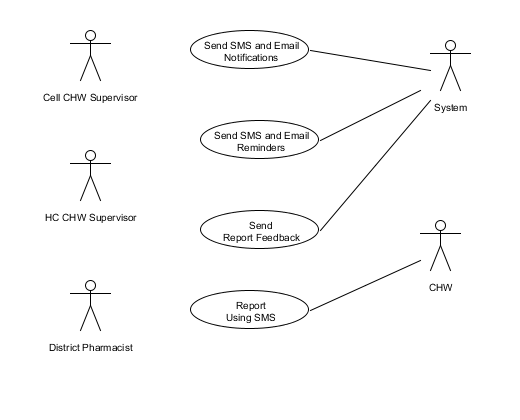
\includegraphics[width=\columnwidth]{img/hmisReq.png}
\label{fig:use_case}
\caption{Use Case Diagram}
\end{figure}


\chapter{Activities}
\section{Setting up the Test Environment}
After defining the use cases we set up a local test environment so that we could check if the use cases was already covered in the latest version of DHIS2, in our case 2.14. This included setting up a local instance of DHIS2 in a Windows based operating system and a SMS gateway in Android.
From testing with the local instance we found that it was already possible to report the essential drugs with a SMS. Also, the system could automatically send user feedback when an SMS is sent.
In the next version of DHIS2 it will be possible to modify the feedback messages so that the Community Health Workers can receive messages in their own language.
We had a short demo for the community help desk to show that objective 3 and 4 were in some way met.
Objective 1 and 2 needed some more work.


\section{Importing users}
We had a csv file of all the community health workers, just under 45,000 users. All of these users needed an user account in the system. In order to do this we made an application that could do this.
This java application essentially creates a password and user name for each user, imports the phonenumber, firstname, surname and assigns them to an org. unit. The application was not nearly finalized, but works for it's purposes. Some security issues were discovered while making this application. Like, DHIS2 still uses the md5 hash to store passwords, rumors has it that this hash is broken.

\section{Reorder algorithm and SMS/email notifications}
This would be our solution to objective 1 and 2. The reorder algorithm was implemented in MySQL.
From the data reported by the 'community health workers' the algorithm could calculate the estimated quantity needed of each drug.

\begin{eqnarray}
reorder_{n} & = & (amc_{n} \cdot 2) - stk_{n} \\
amc_{n} & = & \frac{disp_{n-2} + disp_{n-1} + disp_{n}}{3} \\
disp_{n} & = & stk_{n-1} + rcd_{n} - stk_{n} \\
disp_{n-1} & = & stk_{n-2} + rcd_{n-1} - stk_{n-1} \\
disp_{n-2} & = & stk_{n-3} + rcd_{n-2} - stk_{n-2} \\
\end{eqnarray}

\begin{description}
\item[\textbf{reorder:}]
	This is the quantity of a specific drug that needs to be reordered. This value is calculated based on the previous month. As of writing, the current month is May. This means that \(n=4\). Based on this, the village that reported this data should receive \(reorder_{4}\) of the essential drug in question.
\item[\textbf{amc:}]
	Short for average monthly consumption. In our case it is the average of the dispensed the last 3 months.
\item[\textbf{stk:}]
	Stock at the end of the month of the drug in question. Should be reported by the community health workers.
\item[\textbf{disp:}]
	How much a village has dispensed of the essential drug in \(month_{n}\). This value is calculated by the system. 
\item[\textbf{rcd:}]
	How much a village has received of the essential drug. This is the sum of the how much of the essential drug that are received during \(month_{n}\). 
\end{description}

With these values we would like to have DHIS2 to produce reports that could be sent out to users of the system by SMS and Email triggered by some values. We have not yet figured out how to do this, but it is very likely supported. 

\chapter{Product}
With this report comes two programs that are runnable, but not finished.
\section{User Importer}
The user importer is used to create users in DHIS2 from a csv file in postgresql database.
The output of the application is:
\begin{itemize}
	\item New users in the DHIS2 instance.
	\item (Optional) A csv file containing the username, password, firstname, surname, phonenumber and assigned organization unit for each user.
	\item (Optional) A csv file containing all the records that are missing fields.
\end{itemize}

\section{The Essential Predictore}
This application can run the algorithm discussed earlier. The program still needs modifications, as we are still receiving new requirements from the clients. The core of the program is written in MySQL, and are to advanced for me to make any real description of. The last days of my stay I was trying to make a Java user interface in order to run the program, but have not yet finished.

\chapter{Next steps}
\section{Requirements}
I would strongly suggest that a final requirements document is made. Were every requirement are stated measurable. By continuing to change or add to the requirements it is very difficult to have an overview of the project and the progress. 

\section{SMPP}
In order to support the SMS service I was advised to use the SMPP protocol. For some reason it is difficult to get support for this. Other options are available, but I have not looked into the details. One important step is therefore to get support for SMPP.


\section{Developer in HMIS}
I would strongly suggest that the HMIS team gets a Java developer on site.

\section{DHIS2 Applications}
The applications should be made as DHIS2 applications. I would suggest that me and one team member from the HMIS makes these. I do not have any time available until after august 2014, but are available after this.

\section{Validation rules}
In order to support sending reminders and orders one needs to configure the DHIS2. This requires some knowledge about DHIS2 and how it works. I would suggest that one team member is made responsible for making this happen. The DHIS2 users and developers can be used for support.


\end{document}
